\documentclass[a4paper,oneside,11pt]{article}
\usepackage{cprform_lett}
\usepackage{amsmath,amstext,amsfonts,amsbsy,amssymb,amscd,bbm,epsfig}
\usepackage{lscape,color,multirow,hyperref, url}
\begin{document}


%%%%%%%%%%%%%%%%%%%%%%%%%%%%%%%%%%%%%%%%%%%%%%%%
% TITLE

\noindent\textsf{\Large A unitary SEIR model with turtles}
\vskip 2truemm
\thicktablerule
\vskip 2truemm
\noindent{\large P. Hern\'andez, Carlos~Pena, JJGC \hfill May 2020}
\vskip 10truemm

\section{Introduction}

A burgeoning number of papers have been published over the last few months in the context of the huge scientific effort to understand the current COVID-19 pandemics \footnote{See for example, the CMMID repository, \url{https://cmmid.github.io/topics/covid19/}}. Among these, a large fraction corresponds to papers attempting to model the dynamics of the epidemics. Two main approaches are used in such modelling efforts. One of them, called ABM (agent based models) is based in a microscopic approach in which individual ``agents'' are allowed to interact under some circumstances ---often described by a spatial grid, a connection network or both--- and the parameters of the infection are obtained as ``macroscopic measurements'' of such interactions (much in the same way that pressure and temperature characterise the interaction of molecules in a gas) \cite{Hunter2017}.  A second approach is based in obtained deterministic solutions to a set of differential equations (DEM or differential equation models) which purportedly capture the dynamics of the disease\cite{Hethcote2000}. While ABMs are a relatively new approach, DEMs have been used for almost 100 years, since the original formulation of the SIR (susceptible - infected - recovered) model by Kermack and McKendrick \cite{Kermack1927}. In particular, the so called SEIR (susceptible - exposed - infected - recovered) models have been extensively used in epidemiology \cite{Hethcote2000}, both in the past and in the context of the current crisis \cite{Tang2020}.

It has been recently pointed out that SEIR models fail to describe properly the delay introduced by the incubation time of the disease \cite{fodor2020integral}. As an alternative to DEMs the authors of \cite{fodor2020integral} propose integral equation models. 

Prompted by these observations as well as by the imperious need to better understand the tools used for modelling and forecasting, given their potential impact in decision-making policies, this paper presents a new formulation of the SEIR problem, which we call uSEIR (where the u stands for Unitary) in which a new set of differential equations is deduced from first-principles. We use an ABM calculation to demonstrate that the results of uSEIR are matched by a microscopic simulation of a fully homogeneous, fully susceptible population in the deterministic limit (e.g, with no stochasticity in the model parameters). Furthermore we show that the classic SEIR solution does not match the ABM result. We then obtain the limit in which uSEIR and SEIR converge. This turns out to be the case in which both the incubation and recovery time are assumed to be distributed exponentially. Given the fact that such assumption does not appear to be realistic ---the data is much better described by gamma, lognormal of Weibull distributions---, we also conclude that the use of classic SEIR model does not appear to be justified. 


\section{Unitary SEIR model}
We start by considering a model with compartments for susceptible, exposed, infected and recovered individuals at any given time $t$. To be precise we define these categories
as:
\begin{itemize}
\item $S(t)$: number of susceptible individuals at time $t$.
%that is those that can be infected if in contact with an infected 
\item $E(t)$: number of exposed individuals at time $t$, that is those that will become infected after an incubation time,$t_i$. 
%Note that the exposed individuals that will never become infected are part either of susceptible\footnote{Of course there could be individuals that are immunized, but those are out of the count, there are not part of any category that matters here. }
\item $I(t)$: number of individuals at time $t$ that can infect other people. They remain in this category for time $t_r$. This time might be the natural time of recovery or the time it takes to isolate the individual (thus this category is sometimes also dubbed ``removed'' in addition of the more usual ``recovered''). 
% it is in any case the time that it takes for an infected individual to stop infecting, at that moment the individual is declared recovered.
\item $R(t)$: number of recovered (or removed) individuals.
% that contain any individual that was infected in the past and is no longer infectious either because it died, fully recovered or fully isolated so that its probabilty to infect is zero.
\end{itemize}
There is a unitarity condition in this model.  Each individual must be in one of the S,E,I or R categories. Therefore the number of (non-immunised) individuals in the population, $N$, is a constant:
\begin{eqnarray}
S(t)+ E(t)+I(t)+R(t) = N.
\end{eqnarray}
But there must also be a relation between the rates at which these different individuals move from one category to the next. An infection process is that in which an infected individual gets in contact with a susceptible one. Let us call $r_{S\rightarrow E}$ the rate of infection per unit time
per infected individual and per susceptible individual. The number of susceptible individuals gets reduced by those that become exposed between $[t, t+dt]$, that is:
\begin{eqnarray}
d S(t) = - r_{S\rightarrow E} I(t) S(t) dt.
\label{eq:basic}
\end{eqnarray}
In the simplest approximation, if the incubation and recovery time of all individuals have the same values, then we must also have that the individuals that become exposed at time 
$t$ are those that move from category $S\rightarrow E$ at time $t$ minus those that move from $E\rightarrow I$. But the latter must be the ones that entered the exposed category in time $t-t_i$. Therefore we have:
\begin{eqnarray}
d E(t) &=& -d S(t) + d S(t-t_i) \theta(t-t_i) ,\nonumber\\
d I(t) &=& -d S(t-t_i) \theta(t-t_i)+ d S(t-t_i-t_r) \theta(t-t_i-t_r),\nonumber\\
d R(t) &=& - d S(t - t_i - t_r) \theta(t-t_i-t_r).\nonumber
\label{eqs:cor}
\end{eqnarray}

The initial conditions to these equations start with a fixed $N$ and a number of infected individuals at time $t=0$, $I[0]$, so that $S(0) = N-I(0)$, while $E(0)=0$ and $R(0)=0$.  
In the  equations above, the number of initially infected individuals does not recover, but we can easily force this with the substitution in eq.~(\ref{eq:basic}):
\begin{eqnarray}
I(t) \rightarrow \tilde{I}(t) \equiv I(t) - I(0) \theta(t-t_r).
\end{eqnarray}
These equations depend only on three variables, namely $r_{S\rightarrow E}$, $t_i$ and $t_r$, which in principle are the same parameters appearing in the classical SEIR.
The basic reproduction number, $R_0$, defined as the average number of individuals infected by any given infected individual in a fully susceptible population corresponds to the combination:
\begin{eqnarray}
r_{S\rightarrow E} = {R_0\over N t_r}. 
\end{eqnarray}

Since $R_0$ is clearly proportional to $t_r$, it follows that $r_{S\rightarrow E}$ is not. In a microscopic description of the infected process we expect that the rate $r_{S\rightarrow E}$ is basically the product of the number of contacts per unit time and the probability of infection per contact. 

The result of the classical SEIR and the unitary SEIR model introduced above is very different. Fixing the three parameters to the same values, the two are compared in Fig.~\ref{fig:seirvsuseir}. The differences are stricking. 
\begin{figure}[h!]
  \centering
  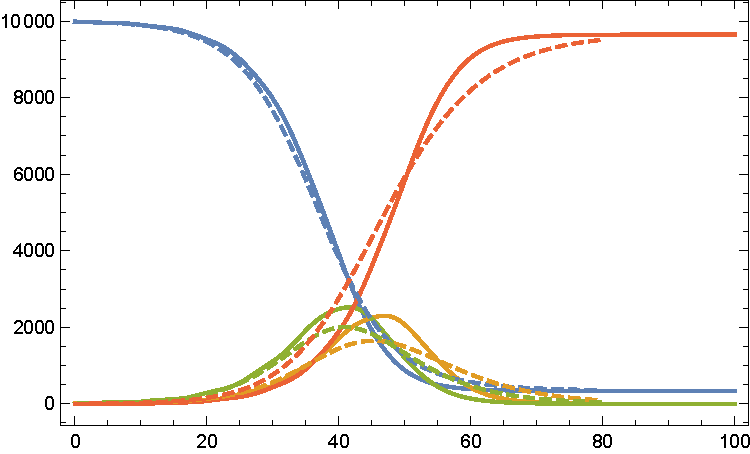
\includegraphics[width=8cm]{seirvsuseir.pdf}
  \caption{ Result from the uSEIR (solid) and classical SEIR(dashed) in a  population of $N=10^4$ and $I(0)=10$ with $R_0=3.5$, $t_i=5.5$ and $t_r=5$. The curves correspond to 
  susceptible (blue), exposed (green), infected (yellow) and recovered (red).  }
  \label{fig:seirvsuseir}
   \end{figure}  
   However, SEIR assumes that the times $t_i$ and $t_e$ are averages, that is they are not uniform in the population. 
          
\subsection{Non-uniform parameters }

In most realistic cases, the parameters will not be uniform across the population. For example, not all individuals have the same incubation or recovery period and certainly not all individuals have the same number of contacts and probability of infection per contact. To try to understand how to treat this possibility the simplest is to consider that within each category there are subcategories of individuals. For example, the susceptible divide themselves into individuals that will have different incubation periods, $t_i^{(i)}$,  according to some distribution for example, so we have $S_i(t)$ as the susceptible individuals in the $i$-th subcategory. Each subcategory follows its usual progression $S_i\rightarrow E_i \rightarrow I_i \rightarrow R_i$, but the important point to notice is that a given susceptible individual in subcategory $i$ becomes an exposed individual in subcategory $i$, but can get infected from any infectious individual in any subcategory, $I_j$. If we assume that the capability to infect per unit time is independent on the category. This means that the number of susceptible individuals in category $i$ change as they become exposed according to:
\begin{eqnarray}
d S_i(t) = - r_{S\rightarrow E} I(t) S_i(t) dt.
\end{eqnarray}
and eqs.(\ref{eq:cor}) will still be valid for the exposed, infected and recovered in category $i$, taking the incubation period as that corresponding to this category, $t^{(i)}$. 

Summing over all the categories, the first equation the leads to:
\begin{eqnarray}
d S(t) = - r_{S\rightarrow E} \tilde{I}(t) S(t) dt, 
\end{eqnarray}
while in the others we get
\begin{eqnarray}
d E(t) &=& -d S(t) + \sum_i d S(t-t^{(i)}_i) \theta(t-t^{(i)}_i) ,\nonumber\\
d I(t) &=& \sum_i  \left\{-d S(t-t^{(i)}_i) \theta(t-t^{(i)}_i)+ d S(t-t^{(i)}_i-t_r) \theta(t-t^{(i)}_i-t_r)\right\},\nonumber\\
d R(t) &=& \sum_i \left\{- d S(t - t^{(i)}_i - t_r) \theta(t-t^{(i)}_i-t_r)\right\}.\nonumber
\label{eqs:corint}
\end{eqnarray}
Obviously in the limit of $t^{(i)}$ varying continuously the sum becomes and integral
\begin{eqnarray}
\sum_i  (...) \rightarrow \int dt_i P(t_i) (...), \;\;\; \int_0^\infty dt_i P(t_i) = 1.
\end{eqnarray}
We can similarly assume subcategories for varying $t_r$ and the modification would be analogous. 

\subsubsection{Recovering classical SEIR}

The case where the probabilities are exponential, the integro-differential equations can be reduced to regular differential ones, of the classical SEIR type.

 Let's assume 
\begin{eqnarray}
P(t_i) = {1\over \langle t_i\rangle} e^{-t_i/\langle t_i\rangle},
\end{eqnarray}
and define
\begin{eqnarray}
F(t) &\equiv& \int_0^\infty dt_iP(t_i) S'(t-t_i) \theta(t-t_i) = \int_0^t dt_i P(t_i)  S'(t-t_i) \nonumber\\
&=& \int_0^t dz P(t-z) S'(z).
\end{eqnarray}
The derivative of this function is related to that of $E(t)$, using eq.~(\ref{eqs:corint}), 
\begin{eqnarray}
F'(t) = {1\over \langle t_i\rangle} \left({d S\over dt}-F(t)\right) = - {1\over \langle t_i\rangle} {dE\over d t}(t), 
\end{eqnarray}
so up to a constant 
\begin{eqnarray}
F(t) = -{E(t)\over \langle t_i\rangle} +C.
\end{eqnarray}
Since $F(0) = E(0) =0$, the constant must vanish and the equations reduce to:
\begin{eqnarray}
{d S\over dt} &=& - r_{S\rightarrow E} \tilde{I}(t) S(t),\nonumber\\ 
{d E\over dt} &=& -{d S\over d t} - {1 \over \langle t_i\rangle} E(t) ,\nonumber\\
{d I\over dt} &=& {1 \over \langle t_i\rangle} E(t) -{1\over \langle t_i\rangle} E(t-t_r) \theta(t-t_r),\nonumber\\
{d R\over d t} &=&  {1\over  \langle t_i\rangle} E(t-t_r) \theta(t-t_r),\nonumber\\
\end{eqnarray}

If we add also an exponential distribution for the recovery time we need the function
\begin{eqnarray}
G(t) \equiv {1\over \langle t_i\rangle } \int dt_r P(t_r) E(t-t_r) \theta(t-t_r), 
\end{eqnarray}
which for an exponential with average $\langle t_r\rangle$ satisfies
\begin{eqnarray}
G'(t) = {E(t)\over \langle t_r\rangle \langle t_i\rangle} - {G(t)\over  \langle t_r\rangle} = {I'(t)\over \langle t_r \rangle},
\end{eqnarray}
and therefore 
\begin{eqnarray}
G(t) = {I(t)\over \langle t_r \rangle} + C,
\end{eqnarray}
where $C= -I(0)/\langle t_r \rangle$.
Finally we also need to average over $t_r$ in the second term of the function $\tilde{I}$:
\begin{eqnarray}
\int d t_r P(t_r) \tilde{I}(t) = I(t) - I(0) \left(1- e^{-t/\langle t_r\rangle}  \right) \equiv \bar{I}(t)
\end{eqnarray}
 So finally the equations are:
\begin{eqnarray}
{d S\over dt} &=& - r_{S\rightarrow E} \bar{I}(t) S(t),\nonumber\\ 
{d E\over dt} &=& -{d S\over d t} -{1 \over \langle t_i\rangle} E(t) ,\nonumber\\
{d I\over dt} &=& {1 \over \langle t_i\rangle} E(t) - {1\over  \langle t_r \rangle} (I(t) -I(0)),\nonumber\\
{d R\over d t} &=&  {1\over  \langle t_r\rangle} (I(t)-I(0)),\nonumber\\
\label{eqs:seirexp}
\end{eqnarray}
which up to the $I(0)$ are the classical SEIR equations. If $I(0)$ is very small, the extra terms 
 can probably be neglected. 

A different situation is found when take subcategories for the rates of infection. In fact, we could separate the population in individuals that infect others with different rates. The rate might depend on the type of infectious individual and the type of susceptible individual. That is $r^{j}_{i}$ would be the rate at which an infected individual of type $j$ infects a susceptible
individual of type $i$. The equations in this case would become:
\begin{eqnarray}
d S_i(t) &=& - \sum_j r^j_{i}  I_j(t) S_i(t) dt, \nonumber\\
d E_i(t) &=& -d S_i(t) + d S_i(t-t_i) \theta(t-t_i) ,\nonumber\\
d I_i(t) &=& -d S_i(t-t_i) \theta(t-t_i)+ d S_i(t-t_i-t_r) \theta(t-t_i-t_r),\nonumber\\
d R_i(t) &=& - d S_i(t - t_i - t_r) \theta(t-t_i-t_r).\nonumber
\end{eqnarray}
where $t_i$ and $t_r$ might also depend on the category.

 In this case, the number of equations is larger. Even in the simplified case where the rates only depend on the type of infecting individual and not on the type of susceptible and for simplicity $t_i$ and $t_r$ are the same, there are two functions $I(t)$ and $\sum_j r^j I_j(t)$ that enter. If we assume that the the different categories are in some proportion and that this proportion is maintained by the initial conditions of the $I_i(0)$ and $S_i(0)$, in this case the proportion should not change in the evolution. If this is so, the equations reduce to the usual ones with a rate that is the weighted average:
 \begin{eqnarray}
 r_{\rm eff} = \sum_i r^i p^i,
 \end{eqnarray}
 where $p^i$ is the proportion of individuals in category $i$.
 
 \subsection{Time-varying parameters}
 
 The parameters of the epidemic might not be uniform, because they change in time or across the population and in genera both, as measures are taken to 
 fight the spread of the epidemic. This is an essential effect since it should modify in a drastic way the height of the peak of infected population that would otherwise
 be controlled by the herd inmmunity which is typically much larger. 

In the previous model it is easy to include a possible time varying function $r_{S\rightarrow E}(t)$, as will be typically the case in an epidemic when isolation measures are taken, which typically reduce the number of contacts per unit time (ie. keeping people isolated) or the probability of infection per contact (ie. wearing masks) or both. 


\section{Agent Based Simulations} 

A number of software packages are available to simulate a epidemic 


\section{uSEIR versus Turtles}

\subsection{Uniform Parameters}

We first compare the result of the uSEIR, the standard SEIR with the average of 10 simulations for the case where all the basic parameters are constant, $t_i$, $t_r$ and $r_{S\rightarrow E}$. 
In Fig.~\ref{fig:fixed} we show the curves for the infected individuals from the three methods, for two values of the fraction $I(0)/N$, 

\begin{figure}[h!]
  \centering
  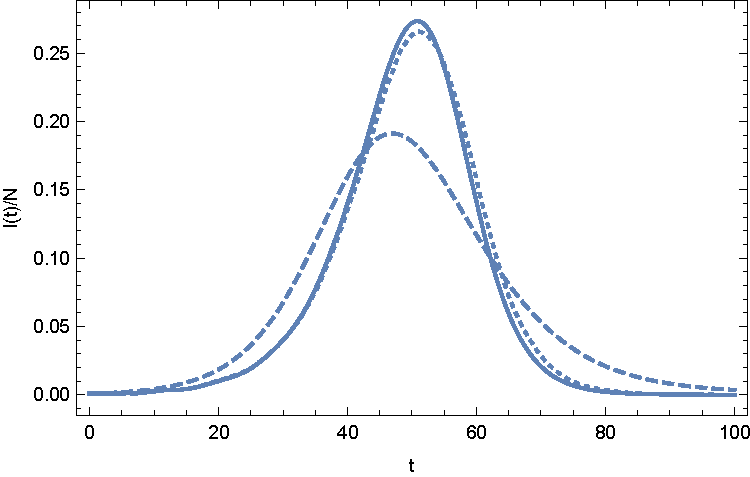
\includegraphics[width=8cm]{fixed.pdf}
  \caption{ Curve of the infected individuals as a function of time for the uSEIR (solid), classical SEIR(dashed) and the agent simulation (dotted) in a  population of $N=10^4$ and $I(0)=10$ with $R_0=3.5$, $t_i=5.5$ and $t_r=6.5$.  }
  \label{fig:fixed}
   \end{figure}  

\subsection{Non-uniform Parameters}

We start by considering the exponential distributions for $t_i$ and $t_r$, while we maintain the rate of infection constant. The comparison of the SEIR solution of eqs.~(\ref{eqs:seirexp}) and simulations are shown in Fig.~\ref{fig:exp}, where the agreement is quite good. 
\begin{figure}[h!]
  \centering
  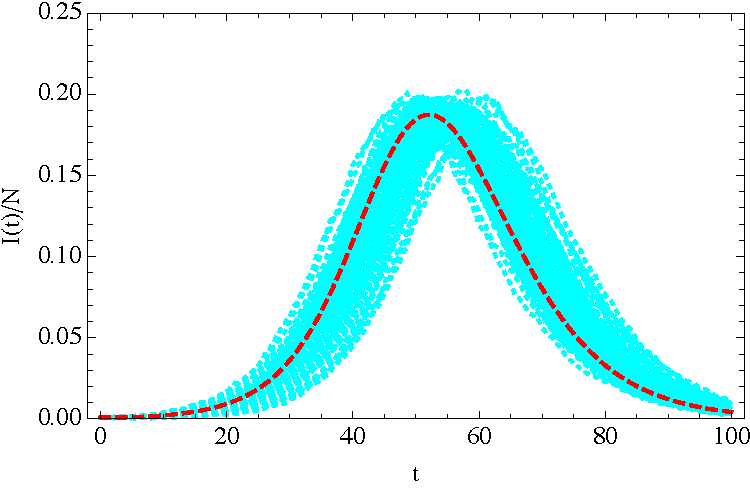
\includegraphics[width=8cm]{expseir.pdf}
  \caption{ Curve of the fraction of infected individuals as a function time of the classical SEIR (solid) of eqs.~(\ref{eqs:seirexp}) and the average of 10 agent simulations (dotted-red) and $10^2$ agent simulations (dotted-blue) 
  in a  population of $N=10^4$ and $I(0)=10$ with $R_0=3.5$, $\langle t_i\rangle=5.5$ and $\langle t_r\rangle=6.5$.  }
  \label{fig:exp}
   \end{figure}  
    Assuming an exponential distribution for the incubation and recovery times are not realistic. A more realistic distribution seems to be the  gamma distribution, $\Gamma[k,\theta]$ \cite{}. For the Covid19 epidemic the parameters have been estimated to be $(k,\theta) \simeq (5.8, 0.948)$, corresponding to an average $\langle t_i\rangle \simeq 5.5$days. For the recovery time we assume the same distribution with parameters $(6.5,1)$.

We compare the results of the simulations with the exponential and gamma distributions in Fig.~\ref{fig:expvsgamma}. We also include the result of solving discretely the eqs.~(\ref{eq:corint})
\begin{figure}[h!]
  \centering
  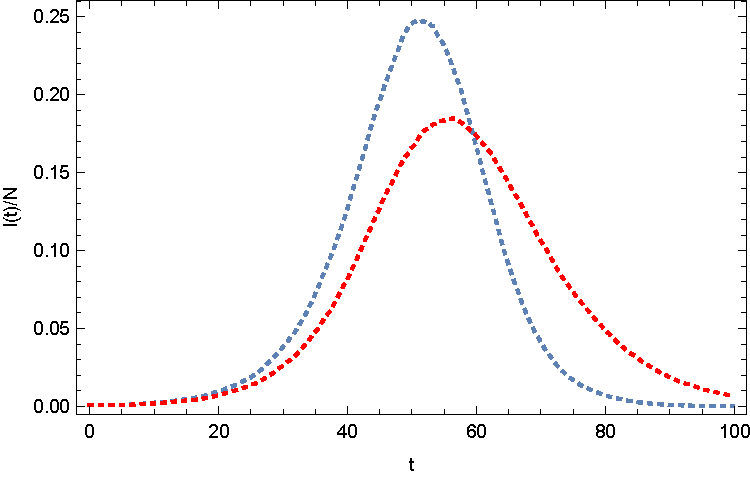
\includegraphics[width=8cm]{expvsgamma.pdf}
  \caption{ Curve of the fraction of infected individuals as a function time from the average of 10 agent simulations with $t_i$ and $t_r$ distributed in the population according to the gamma distributions (blue) and exponentials (red). The simulation has parameters in both cases $N=10^4$ and $I(0)=10$ with $R_0=3.5$, $\langle t_i\rangle=5.5$ and $\langle t_r\rangle=6.5$.  }
  \label{fig:exp}
   \end{figure}  
   
   The evolution of the epidemic is very different even if the total number of non-infected individuals  is quite similar. This is generically the case when the rate of 
   infection is uniform in the population and $R_0 >1$. In practice $R_0$ will also  be non-uniform. Particularly important are the fraction of individuals for which the probability of infecting is zero, which in practice makes them immune. Their presence in a given population implies that the effective number of useful contacts gets reduced. The fraction of the population with zero infecting power is equivalent to the inmune fraction. When this fraction is large enough the effective $R_0$ can be below 1 and therefore the epidemic may not start. This is the concept of herd inmunity, used to measure the fraction of vaccinated population that can abort an epidemic. A very rough estimate for the fraction of herd immunity, $f_I$, would be
   \begin{eqnarray}
  R_0 (1- f_I)  =1, \;\; f_I= 1-1/R_0. 
   \end{eqnarray} 
   For Covid19, with $R_0 \sim 3$, $f_I \sim 0.7$, that is $70\%$ of the population. One would naively estimate then that in a given epidemic with this herd immunity would result in a 
 fraction of  population that gets infected at some point of 70$\%$, but what we have seen is that the fraction is much larger, both in the SEIR equations as in the simulations. This is because of the time delay in the process, the fraction of recovered individuals grows slowly and is not effective in reducing the growth of the epidemic sufficiently, as if the fraction of immune individuals would be there from the start. 
 
 The non-uniformity of $R_0$ is however very important. It has been argued that for Covid19 this distribution of this quantity is well described by the negative binomial distribution, $NB[0.16,0.0437]$, which has average 3.5 but a large dispersion. This distribution implies that about $60\%$ of the population would not infect anyone (not far from the naive herd immunity), while there must be few individuals that have a very large rate of infection, the superspreaders. One can get an idea of the relevance of the distribution in $R_0$ by solving the uSEIR equations changing the value of $R_0$  as drawn from the averages over the population with $N$ individuals. This is shown on the left of Fig.~\ref{fig:dispersion}. Each curve correspond to the the uSEIR equations with $R_0$ being the average over the population. Since this average has some variance, the curves evolve differently. However much more important is the effect of the initial conditions, which are completely non-universal. We can mimic this effect by measuring the average $R_0$ of the 10 initially infected individuals.  We can simply take the rate of infection to be this value for $t< tr$ and change to the population average after this time (in reality the evolution will be more smooth of course). The effect of this is shown on the right Fig.~\ref{fig:dispersion}. The history of each epidemic is strongly dependent on the initial conditions which are quite random. It is not clear what we gain 
 from the average, since each epidemic will have a unique starting point. 
\begin{figure}[h!]
  \centering
  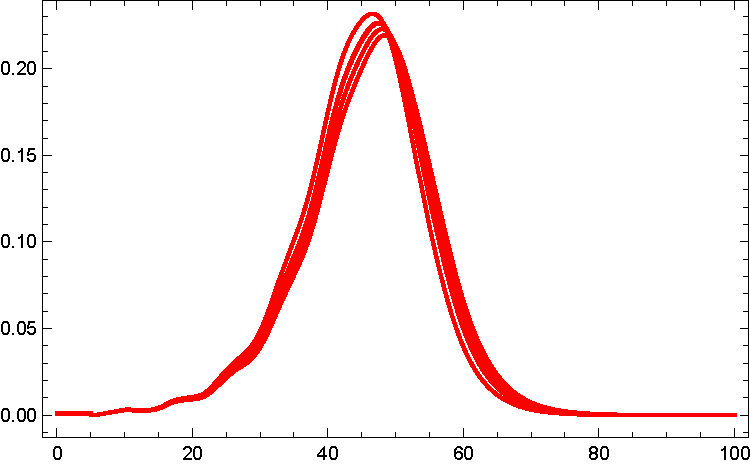
\includegraphics[width=7cm]{NBdisR0.pdf}   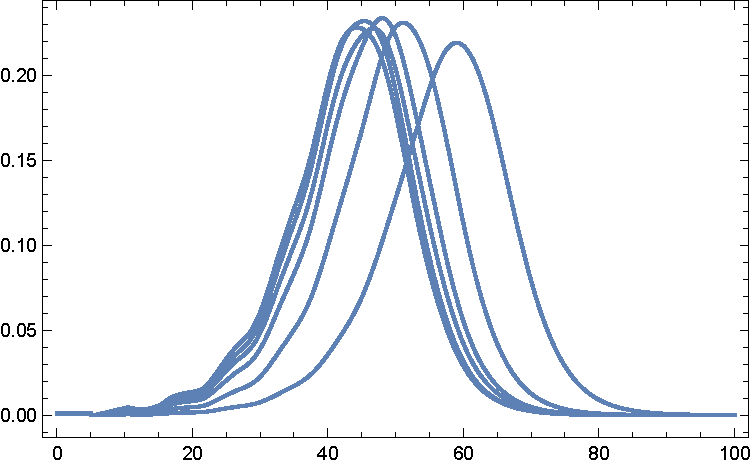
\includegraphics[width=7cm]{NBdisR00.pdf}
  \caption{ Left: Curve of the fraction of infected individuals as a function time resulting from the uSEIR equations  for fixed $t_i =5.5$ and $t_r=5$ with $N=10^4$ and $I(0)=10$ and $R_0$ drawn from the average of the $N$ population. Right: the same but assuming that the rate  $R_0$ for $t<t_r$  is the average over the 10 individuals that start the epidemic and for later time the rate turns to the average. }
  \label{fig:dispersion}
   \end{figure}  
   
 We have observed however, that the main effect of the different initial conditions is a temporal shift of the maximum but the shape or the height of the infection curve does not change significantly. This strongly suggest that the equations have a universal solution. We have indeed found it. Let's assume we consider the differential equations eqs.~\ref{} near the maximum of the infection curve $t_{\rm max}$, which will remain as a free parameter. Let's also assume that $t_{\rm max} \gg t_i, t_r$ and let's define the function
 \begin{eqnarray}
 F(t) \equiv S(t) I(t).
 \end{eqnarray} 
 The diferential equations for the uSEIR with fixed $t_i$ and $t_r$ and for $t\gg t_i, t_r$:
 \begin{eqnarray}
 {d S \over dt}+{d R\over dt} &=& r F(t-t_i - t_r) - r F(t) \simeq -r (t_i+t_r) {dF(t)\over dt}, \nonumber\\
  {d E \over dt} &=& r (F(t) - F(t-t_i))  \simeq r t_i {d F(t) \over dt}, \nonumber\\
   {d I \over dt} &=& r (F(t-t_r) - F(t-t_i-t_r))  \simeq r t_r {d F(t-t_i) \over dt}.
 \end{eqnarray}
 which implies
 \begin{eqnarray}
 S(t)+R(t) &=& C - r (t_i + t_r) F(t), \nonumber\\
   E(t) &=& C' +r t_iF(t), \nonumber\\
   I(t) &=& C'' +r t_r F(t-t_i). \;\;
 \end{eqnarray}
 Since $I(t) \rightarrow 0, E(t)\rightarrow 0, F(t) = S(t) I(t) \rightarrow 0$ as $t\rightarrow \infty$, it follows that $C'=0, C''=0$ and $C= N$. 
 
 Using the previous equations, it is easy to derive the differential equation for $F(t)$, expanding at linear order in $t_i$ and $t_r$:
 \begin{eqnarray}
 F'(t)&=& S'(t)I(t) + S(t) I'(t)\nonumber\\
 & =& - r^2 t_r  F(t)^2 + \left(1+t_i {F'(t)\over F(t)}\right) \left(F'(t)  -t_i F''(t)\right),\nonumber\\
 & =& - r^2 t_r  F(t)^2  + F'(t)+t_i {F'(t)^2\over F(t)} -t_i F''(t).
 \end{eqnarray} 
 so we finally obtain
  \begin{eqnarray}
 F''(t) - {F'(t)^2\over F(t)} + r^2 {t_r\over t_i} F(t)^2 = 0.  
 \end{eqnarray}
 We are interested in the solution near the maximum, so we use the initial conditions:
 \begin{eqnarray}
 F'(t_{\rm max}) = 0, \;\;\; F(t_{\rm max}) = F_0.
 \end{eqnarray}
 This non-linear equation has a solution which is given by:
\begin{eqnarray}
F(t) = F_0 \left(1 - \tanh^2\left[ a (t-t_{\rm max})\right]\right),
\end{eqnarray} 
with 
\begin{eqnarray}
a\equiv r \sqrt{{t_r\over 2 t_i}} \sqrt{F_0}.
\end{eqnarray}
This is the universal function that drives the evolution of the infected, exposed and susceptible+recovered inviduals near the maximum. The maximum of the infected is at $t_{\rm max}-t_i$ for the infected, while the maximum(minimum) for the exposed(susceptible+recovered) is at $t_{\rm max}$. The integral of this function from $[-\infty, \infty]$ is
\begin{eqnarray}
\int F(t) = {2 F_0 \over a}.
\end{eqnarray}
We can also derive the value of the susceptible at $t_{\rm max}$ since
\begin{eqnarray}
S(t_{\rm max}) = {F(t_{\rm max}) \over I(t_{\rm max})} = {1  \over r t_r  (1- \tanh^2\left[ a t_i\right])}.
\end{eqnarray}
and the curve of the susceptible can be easily obtained 
\begin{eqnarray}
S(t) = S(t_{\rm max}) \exp \left(-r \int_{t_{\rm max}}^t F(t) dt \right).
\end{eqnarray}
which gives the final  susceptible population at the end of the epidemic to be:
\begin{eqnarray}
S(t_\infty) = S(t_{\rm max}) \exp\left(- {r^2 t_r F_0\over a}\right). 
\end{eqnarray}
Finally we can get another expression for $S(t)$ as
\begin{eqnarray}
S(t) = S(t_{\rm max}) - r \int_{t_{\rm max}}^t F(t).
\end{eqnarray}
Requiring that the two are the same at $t_\infty$ gives the following condition on $F_0$:
\begin{eqnarray}
{1-\exp(2 a t_i)\over 1-\tanh^2(a t_i)} = 2 a t_i,
\end{eqnarray}
which has a non-trivial solution
\begin{eqnarray}
a\sim t_i^{-1} \rightarrow F_0 \simeq {2 \over t_r t_i r^2}. 
\end{eqnarray}
With this we conclude that the epidemic curve is universal once the value of the maximum position is determined. 
The only dependence on the initial condition remains in $t_{\rm max}$. 

\subsection{Time-varying Parameters}
\section{Conclusions}

%\end{document}
%
%\title{SEIR de andar por casa}
%
%A ver, he estado intentado entender el asunto del tiempo de incubaci\'on y de recuperaci\'on en el SEIR y he llegado a la conclusi\'on de que 
%no lo entiendo, en particular que el n\'umero de infectados en tiempo $t$ sea proporcional al n\'umero de expuestos en tiempo $t$...
%
%Si hago las siguientes asumptions:
%\begin{itemize}
%\item hay un tiempo de incubaci\'on $t_i$ igual para todos los individuos
%\item hay un tiempo de recuperaci\'on $t_r$ igual para todos los individuos
%\end{itemize}
%las ecuaciones que para m� tendr�an sentido, en t�rminos de unitariedad, son las siguientes:
%\begin{eqnarray}
%{d S\over d t} & = & - \alpha I(t) S(t),\\
%{d E\over d t} & = & \alpha I(t) S(t) - \alpha I(t-t_i) S(t-t_i)  \theta(t-t_i),\\
%{d I\over d t} & = & \alpha I(t-t_i) S(t-t_i) \theta(t-t_i) - \alpha I(t-t_i-t_r) S(t-t_i-t_r)  \theta(t-t_i-t_r),\\
%{d R\over d t} & = & \alpha I(t-t_i-t_r) S(t-t_i-t_r)  \theta(t-t_i-t_r),\\
%\end{eqnarray}
%donde
%\begin{eqnarray}
%\alpha= {R_0\over N t_r} 
%\end{eqnarray}
%En esencia, los que pasan a infectados en tiempo $t$ son los que estaban pasando a expuestos a tiempo $t-t_i$, y los que pasan 
%a recuperados a tiempo $t$ los que estaban pasando a expuestos a tiempo $t-t_i-t_r$...
%
%Comparo con la soluci\'on SEIR (dashed) con supuestamente los mismos par\'ametros donde $t_i$ y $t_r$ si entiendo bien aparecen en los
%rates. Asumo $S[0] = 1000, I[0] =1,  t_r=15,  t_i=5 , \alpha=R_0/t_r = 1/5$.
% \begin{figure}[h!]
%  \centering
%  \includegraphics[width=8cm]{sir.pdf}
%   \end{figure}  
%
%Hay que hacer una peque�a modificaci\'on para que los que est\'an infectados al principio $I[0] = I_0$ decaigan tambi\'en (si no se quedan en el limbo):
%\begin{eqnarray}
%{d S\over d t} & = & - \alpha \tilde{I}(t) S(t),\\
%{d E\over d t} & = & \alpha \tilde{I}(t) S(t) - \alpha \tilde{I}(t-t_i) S(t-t_i)  \theta(t-t_i),\\
%{d I\over d t} & = & \alpha \tilde{I}(t-t_i) S(t-t_i) \theta(t-t_i) - \alpha \tilde{I}(t-t_i-t_r) S(t-t_i-t_r)  \theta(t-t_i-t_r),\\
%{d R\over d t} & = & \alpha \tilde{I}(t-t_i-t_r) S(t-t_i-t_r)  \theta(t-t_i-t_r),\\
%\end{eqnarray}
%with
%\begin{eqnarray}
%\tilde{I}(t) \equiv I(t) - I(0) \theta(t-t_r)\
%\end{eqnarray}
%
%Para incluir una estocasticidad en el valor de $t_i$, a\~nadimos una integral en los t\'erminos de la derecha de la forma
%\begin{eqnarray}
%\int dt_i P(t_i) (...),
%\end{eqnarray}
%donde asumimos un distribuci\'on $\gamma$ con $(k,\theta)=(5.8,0.948)$ \cite{}. En la pr\'actica Mathem\'atica no sabe hacer esto, as\'{\i} que 
%divido la distribuci\'on en tres rangos $[0,t_1], [t_1,t_2], [t_2,\infty]$, con probabilidad $\sim 0.3$ cada uno,  donde tomo la media $\langle t_i\rangle_{1-3}$ en el intervalo y hago la integral como suma 
%de tres t\'erminos:
%\begin{eqnarray}
%\int d t_i P(t_i) f(t_i) \simeq \sum_k f(\langle t_i\rangle_k) \int_{t_k^{min}} ^{t_k^{max}}  P(t_i) 
%\end{eqnarray}
%The comparison of the evolution of infected with an average $t_i$ or an integral with three ranges is shown in \ref{fig:comp}
% \begin{figure}[h!]
%  \centering
%  \includegraphics[width=8cm]{deltavs3.pdf}
%  \label{fig:comp}
%  \caption{Unitary SEIR with fixed $t_i=5.5$ (solid) or with three ranges according to the $\gamma$ distribution (dashed).}
%   \end{figure}  
%We can do the same for changing $t_r$ instead, while any possible change to $\alpha$ of this form would not modify the result for fixed $\langle \alpha\rangle$. 
%
%What is clear is that if we start with the measured $R_0$, unless there is a change with time of $\alpha$ there 
%
\bibliographystyle{unsrt}
\bibliography{refs}
\end{document}

